\graphicspath{{chapters/18/images/}}
\chapter{Free energy calculations}

The need for Free Energy Calculations arises from the fact that most of the time we need to compare our results with affinities, or binding energies, which are related to free energy.
\section{Free energy perturbation theory}
It's only thanks to free energy differences that we can derive some insight on the system. 
For example, calculate the binding process of the inhibitor of an enzyme. 


\begin{figure}
\centering
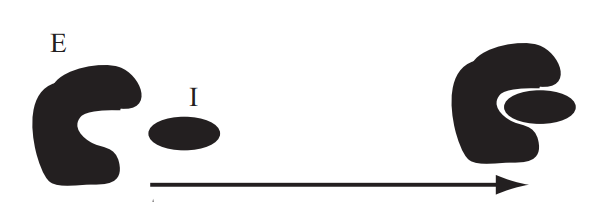
\includegraphics[scale=0.4]{enzymes.png}
\end{figure}

Let's assume there are two states $A$ and $B$.
We can assume that the potential $U_A$ is the interaction-free potential, while the potential $U_B$ the interactions between the enzyme and the inhibitor are taken into account.

$$U_A(\vec{r}_1, \dots, \vec{r}_n)\land U_{B}(\vec{r}_1, \dots, \vec{r}_N)$$

The potential $U_B$ would be the one used in the simulations, while in potential $U_A$ the only way in which the enzyme end the inhibitor could meet is through entropy, e.g. let the water molecules explore all of the configurations.

The free energy difference for state $A$ and state $B$ is:

$$\Delta A_{AB} = -kT\ln Q_B + kT\ln Q_A = -kT\ln\frac{Z_B}{Z_A}$$

Which can be written through the \textit{configurational partition function}, that is the partition function, but with the integration over the momenta already taken.

The two quantities:
$$Z_A = \int d^N\vec{r}e^{-\beta U_A(\vec{r}_1, \dots, \vec{r}_N)}\qquad Z_B = \int d^N\vec{r}e^{-\beta U_B(\vec{r}_1, \dots, \vec{r}_N)}$$

Are extremely difficult to compute. 
We would need to sum over all the possible states to get all of the contributions.
However, there a few tricks that can be used.

Let's write the partition function for state $B$:

$$Z_B = \int d^N\vec{r}e^{-\beta U_B(\vec{r}_1, \dots, \vec{r}_N)} = \int d^N\vec{r}e^{-\beta[U_B(\vec{r}_1, \dots, \vec{r}_N)-U_{A}(\vec{r}_1, \dots, \vec{r}_N)]}e^{-\beta U_A(\vec{r}_1, \dots, \vec{r}_N)}$$

In the second equality we just multiply by the Boltzmann factor for state A.
We can easily write the following equality:

$$\frac{Z_B}{Z_A} = \frac{1}{Z_A}\int d^N\vec{r}e^{-\beta[U_B(\vec{r}_1, \dots, \vec{r}_N)-U_{A}(\vec{r}_1, \dots, \vec{r}_N)]}e^{-\beta U_A(\vec{r}_1, \dots, \vec{r}_N)}$$

The difference in energy between the states is then:
$$\Delta A_{AB} = -kT\ln\frac{Z_B}{Z_A}\qquad\frac{Z_B}{Z_A} = \biggl\langle e^{-\beta[U_B(\vec{r}_1, \dots, \vec{r}_N)-U_A(\vec{r}_1, \dots, \vec{r}_N)]}\biggr\rangle_A$$

Free energy perturbation formula (Zwanzig, 1954):

$$\Delta A_{AB} = -kT\ln\biggl\langle e^{-\beta[U_B(\vec{r}_1, \dots, \vec{r}_N)-U_A(\vec{r}_1, \dots, \vec{r}_N)]}\biggr\rangle_A$$

The exponent is simply an energy difference, taken from the same force field, by switching off and on the interactions between the two objects of interest (defined by the potentials). 
The difficulty in using this equilibrium is that while sampling the canonical distribution for sate $A$, there's very little probability of finding an overlap between the two states.

In case of poor overlap we use the same formula as before, but applied to each step in this calculation:

$$\Delta A_{AB}=0kT\sum\limits_{\alpha=1}^{M-1}\ln\bigl\langle e^{-\beta\Delta U_{\alpha, \alpha+1}(\vec{r}_1, \dots,\vec{r})N}\bigr\rangle_\alpha$$

The average has to be calculated for every state $\alpha$.
This also means that each simulation is independent from each other (and can be run in parallel).

	\subsection{Adiabatic switching}
Instead of using a discretized version of the free energy perturbation, we can apply a switching function tot he two potentials.
The resulting potential is a combination of the potential describing state $A$ and the one describing state $B$:
	$$U(\vec{r}_1, \dots, \vec{r}_N, \lambda) \equiv f(\lambda)U_A(\vec{r}_1, \dots, \vec{r}_N)+g(\lambda)U_B(\vec{r}_1, \dots, \vec{r}_N)$$
	
	We can define the function $\lambda$ as:

	$$f(0) = 1, \quad f(1) = 0,\quad g(0) = 0, \quad g(1) = 1$$
	
	The partition function (from the canonical ensemble) now will depend on $\lambda$:

	$$Q(N, V, T, \lambda) = C_N\int d^N\vec{p}d^N\vec{r}e^{-\beta\biggl[\sum\limits_{i=1}^N\frac{\vec{p}_o^2}{2m_i}+U(\vec{r}_1, \dots, \vec{r}_N, \lambda)\biggr]}$$
Also the Helmholtz free energy will depend on $\lambda$:
	$$A(N, V, T, \lambda) = -kT\ln Q(N, V, T, \lambda)$$
	
	What if we take the derivative of the Helmoltz free energy wet $lambda$?
	The derivative is:

	$$\frac{\partial A}{\partial \lambda} = -\frac{kT}{Q}\frac{\partial Q}{\partial \lambda} = -\frac{kT}{Z}\frac{\partial Z}{\partial\lambda}$$
	
	Since $\lambda$ only appears in the potential and not on the kinetic energy, the derivative can be written as $-\frac{kT}{Z}\frac{\partial Z}{\partial\lambda}$.
	
	The derivative can be written in a better way:

	$$\frac{kT}{Z}\frac{\partial Z}{\partial \lambda} = \frac{kT}{Z}\frac{\partial}{\partial\lambda}\int d^N\vec{r}e^{-\beta U(\vec{r}_1, \dots, \vec{r}_N, \lambda)} = \frac{kT}{Z}\int d^{N}\vec{r}\biggl(-\beta\frac{\partial U}{\partial\lambda}\biggr)e^{-\beta U(\vec{r}_1, \dots, \vec{r}_N)} = -\biggl\langle\frac{\partial U}{\partial\lambda}\biggr\rangle$$

	At the end we get the derivative of $U$ wrt $\lambda$. One trivial function that satisfies the first relation would be, for example, a function that is $f = 1-\lambda$ and $g = \lambda$. 
	For such a  function, the adiabatic switching looks like the Zwanzig's procedure, but we can use any function.
	

	\subsection{Thermodynamics integration}

	The free energy difference between $A$ and $B$ can be defined as the formula below, using the result from the adiabatic switching:

	$$\Delta A_{AB} = \int_0^1\biggl(\frac{\partial A}{\partial \lambda}\biggr)d\lambda = \int_0^1\biggl\langle\frac{\partial U}{\partial\lambda}\biggr\rangle_\lambda d\lambda$$
	There are many ways in which integrals can be computed, e.g. \textit{Gaussian Quadrature}, which gives the best approximation for a small number of points.
	In this case, every value of $\lambda$ would be an independent run of a simulation, so many simulations can be run at the same time and use the found points to calculate the integral. 
	There's however another method: thermodynamic integration.
	The aim of the method is to make the region between $\lambda=0$ and $\lambda=1$ energetically unfavorable.
	Indeed, the difference between the energy of the states only depends on the initial and final state and does not depend on the route the system takes to make such a transition.
	\begin{figure}[H]
		\centering
		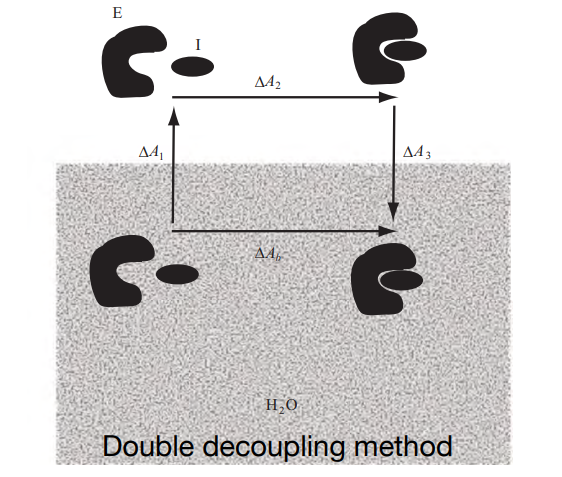
\includegraphics[scale=0.5]{ddm.png}
		\caption{Representation of two thermodynamic pathways for the calculation of the binding free energy of an enzyme E and inhibitor I. According the figure $\Delta A_b = \Delta A_1 + \Delta A_2 + \Delta A_3$}
		\label{fig:ddm}
	\end{figure}
	
	In the real case, some water molecules may affect the dynamics of the system and we cannot arbitrarily remove all the molecules of the solvent.
	
	\subsection{Adiabatic Free Energy Dynamics}
	There are several other methods to calculate the free energy difference.
	For the methods seen before, the difference between all of the states in the middle of the two states of interest have to be calculated.
	We would like instead to explore more the states $A$ and $B$.
	In Adiabatic Free Energy Dynamics, $\lambda$ becomes a variable in the hamiltonian (with associated momenta).

	$$\mathcal{H}_\lambda(\vec{r}, \lambda, \vec{p}, p_\lambda) = \frac{p_\lambda^2}{2m_\lambda} + \sum\limits_{i=1}^N\frac{\vec{p}_i^2}{2m_i} + U(\vec{r}_1, \dots, \vec{r}_N, \lambda)$$

	In the partition function, we integrate also over the values of $lambda$:
	$$Q(N, V, T) = \int dp_\lambda\int d^N\vec{p}\int_0^1d\lambda\int d^N\vec{r}e^{-\beta\mathcal{H}_\lambda(\vec{r},\lambda,\vec{p}, p_\lambda)}$$

	The probability distribution is $P(\lambda') = \langle\delta(\lambda-\lambda')\rangle$. 
	Once we have the probability distribution we can define the \textbf{free energy profile}: $A(\lambda') = -kT\ln P(\lambda')$. 
	This free energy profile would be negative only with very high value of $P(\lambda ')$, e.g. a deep well in the potential.
	
	$P(1)$ would be the partition function for state $B$, and $P(0)$ would be the partition function for state $A$:

	$$A(1) = A(0) = -kT\ln\frac{P(1)}{P(0)} = -kT\ln\frac{Q_B}{Q_A} = \Delta A_{AB}$$


	\begin{figure}[H]
		\centering
		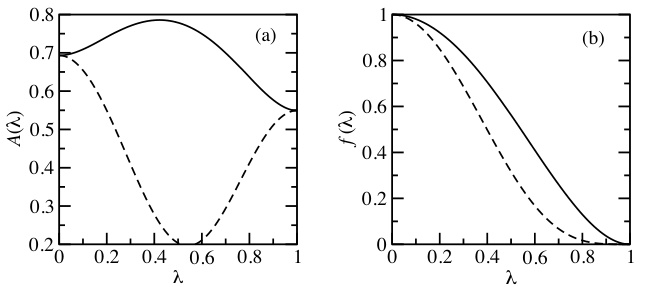
\includegraphics[scale = 0.5]{adiabatic-free-energy-dynamics}
		\caption{\textbf{(a)} Free energy profiles. The solid line indicates switches
$f(\lambda) = (\lambda^2 - 1)^2$ and $g(\lambda) = ((\lambda - 1)^2 - 1)^2$, and the dashed line indicates $f(\lambda) = (\lambda^2 - 1)^4$ and $g(\lambda) = ((\lambda - 1)^2 - 1)^4$ . \textbf{(b)} Corresponding switch $f(\lambda)$.}
		\label{fig:adiabatic-free-energy-dynamics}
	\end{figure}

	In figure \ref{fig:adiabatic-free-energy-dynamics}(a) we can see the energy profiles for different functions. 
	The free energy difference is the same for the two methods, but the profile is very different.
	In the profile that displays a minimum, we expect to be spending more time away from the configurations of interest, in regions which are not physical. 
	In the second case, which shows a maximum point, the configurations in which we spend more time are the ones closer to $\lambda = 0$ and $\lambda = 1$. 
	
	If the system has a barrier $U^{\ddagger}$, the probability to cross a barrier $U^{\ddagger}$ is proportional to $e^{-\frac{U^{\ddagger}}{kT}}$.
	
	In Adiabatic free energy dynamics the idea is to raise the temperature of the $\lambda$ degree of freedom: $\biggl\langle\frac{p_\lambda^2}{2m_\lambda}\biggr\rangle = kT_\lambda$.
	The term $lambda$ is now very hot, more than the actual temperature at which we want to simulate the system.
	However, this makes $\lambda$ fluctuate a lot, which is not desirable, so we also increase its mass.
	This is called adiabatic decoupling: it increases $m_\lambda$ until the $\lambda$ degree of freedom is decoupled from all other degrees of freedom. 
	Now $\lambda$ is almost fixed:

	$$Z(\lambda, \beta) = \int d^N\vec{r}e^{-\beta U(\vec{r}, \lambda)}\qquad\text{ Correct if }\lambda\text{ is fixed}$$
	
	The temperature $\beta$ is the temperature at which we want to simulate the system.
	Because of decoupling, we assume that in the simulation there's enough time for the system to equilibrate and to explore all its possible conformations in a particular value of $\lambda$

	We can now define the\textbf{ potential of mean force} in $\lambda:-\frac{1}{\beta}\ln Z(\lambda, \beta)$.
	
	Because of adiabatic decoupling, $\lambda$ moves quasi-independently from the physical degrees of freedom in the potential of mean force, subject to an effective Hamiltonian:

	$$\mathcal{H}_{eff}(\lambda, p_\lambda) = \frac{p_\lambda^2}{2m_\lambda} -\frac{1}{\beta}\ln Z(\lambda, \beta)$$ 
	
	In this hamiltonian, the kinetic energy is thermostatted by $\lambda$ and the potential of mean force acts as a potential. 
	Notice that in this hamiltonian the potential depends on the temperature, which is usually not the case (this is the reason why it is an "effective" hamiltonian). 
	

	$\lambda$ is thermostatted at a temperature $T_\lambda>T$, hence the obtained canonical distribution ($adb$ because it is obtained through decoupling) is:

	$$P_{adb}(\lambda, p_\lambda, \beta, \beta_\lambda)\propto e^{-\beta_\lambda\mathcal{H}_{eff}(\lambda, p_\lambda)}$$
	
	If we want to obtain the probability distribution for $\lambda$ we need to integrate over $p_{lambda}$:

	$$\tilde{P}_{adb}(\lambda, \beta, \beta_\lambda) = \int dp_\lambda P_{adb}(\lambda, p_\lambda, \beta, \beta_\lambda)\propto e^{\beta_\lambda\ln \frac{Z(\lambda, \beta)}{\beta}} = [Z(\lambda, \beta)]^{\frac{\beta_\lambda}{\beta}}$$
	
	If we take the free energy profile for the probability distribution $[Z(\lambda, \beta)]^{\frac{\beta_\lambda}{\beta}}$:

	$$A(\lambda) = -kT_\lambda\ln\tilde{P}_{adb}(\lambda, \beta, \beta_\lambda) = -kT\ln Z(\lambda, \beta) + const$$

	And we get the free energy profile for the temperature at which we want to obtain the free energy difference, and not for the temperature used for the $\lambda$ degree of freedom. 

\section{Jarzynski's equality}
The free energy difference is called in called in this way because there exists the work-free energy inequality: $W_{AB}\ge \Delta A_{AB}$.
In every thermodynamic transformation, the work is equal to $\Delta A_{AB}$ only if the transformation is fully reversible.
To calculate the work, we need an estimator for it.
We want to obtain a quantity that is equal to the free energy difference, no matter which transformation is happening.
$W_{AB}$ is a thermodynamic quantity and can be expressed as a thermodynamic average:

$$W_{AB} = \langle\mathcal{W}_{AB}(x)\rangle$$

Initial distribution of microstates $x_0\in A$.
They can be all the microstates compatible with the conditions that define state $A$, e.g. state $A$ has its own temperature, so the microstates will be weighted by the Boltzmann factor (Canonical distribution).
The work $\mathcal{W}_{AB}(x_0)$ is a functional of the path $\mathcal{W}_{AB}[x_t] = \mathcal{W}_{AB}[x_t(x_0)] = \mathcal{W}_{AB}(x_0)$.
For each microstate, the system will evolve in a different path.

The thermodynamic value for the work is then:
$$W_{AB} = \langle\mathcal{W}_{AB}(x_0)\rangle_A=\frac{C_N}{Q_A(N, V, T)}\int dx_0e^{-\beta\mathcal{H}_A(x_0)}\mathcal{W}_{AB}(x_0)\ge \Delta A_{AB}$$

Jarzynski's theorem states that if instead of calculating the average over all initial conditions $\langle\mathcal{W}_{AB}(x_0)\rangle_A$ we calculate $\langle e^{-\beta\mathcal{W}_{AB}(x_0)}\rangle_A$ (it looks like a Boltzmann weight for the work estimator), then we get exactly $e^{-\beta\Delta A_{AB}}$, whatever the transformation is:

$$\langle e^{-\beta\mathcal{W}_{AB}(x_0)}\rangle_A = \frac{C_N}{Q_A(N, V, T)}\int dx_0e^{-\beta\mathcal{H}_A(x_0)}e^{-\beta\mathcal{W}_{AB}(x_0)} = e^{-\beta\Delta A_{AB}}$$

This equality also hold for irreversible transformations, that can be used to obtain quantities that describe states at equilibrium.
This has huge implication in computational and experimental physics: in practice it is very difficult to design an experiment with a reversible transformation, instead of an irreversible one.

\subsection{Jarzynski's equality Proof}
There are several proofs for Jarzynski's equality theorem, but we will only go through one.
Let's first define:
$$\Delta A_{AB} = -kT\ln\langle e^{-\beta\mathcal{W}_{AB}(x_0)}\rangle_A$$

And the time dependent Hamiltonian: 
$$\mathcal{H}(\vec{r}, \vec{p}, t) = \sum\limits_{i=1}^N\frac{\vec{p}_i^2}{2m_i} + U(\vec{r}, t)$$.

$$\frac{d\mathcal{H}}{dt} = \nabla_{x_t}\mathcal{H}\cdot\dot{x_t}+\frac{\partial\mathcal{H}}{\partial t}$$

$$\int_0^\tau\frac{d\mathcal{H}}{dt} = \underbrace{\int_0^\tau\nabla_{x_t}\mathcal{H}\cdot\dot{x}_tdt}_{\text{Heat}}+\underbrace{\int_0^\tau\frac{\partial\mathcal{H}}{\partial t}dt}_{\text{Work}}$$

If we use hamiltonian dynamics and there are no dissipative forces, the heat factor is equal to zero.
The formula above also represents the first law of thermodynamics.

The estimator for the work is $\mathcal{W}_{t'}(x_0)$:

$$\mathcal{W}_{t'}(x_0) = \int_0^{t'}\frac{\partial\mathcal{H}(x_t(x_0), t)}{\partial t}dt\qquad \mathcal{W}_{AB}(x_0) = \mathcal{W}_\tau(x_0)$$

Notice that if the hamiltonian is not explicitly time-dependent this would be null (no work is done in the system).

If hamilton's equations are used: $\nabla_{x_t}\mathcal{H}\cdot\dot{x}_t = 0\Rightarrow\frac{\partial\mathcal{H}}{\partial t} = \frac{d\mathcal{H}}{dt}$. 
Meaning, the partial time derivative can be substituted with the total time derivative and the integral can be calculated quite easily: 

$$W_{t'}(x_0) = \int_0^{t'}\frac{\partial\mathcal{H}(x_t(x_0),t)}{\partial t}dt = \int_0^{t'}\frac{d\mathcal{H}(x_t(x_0), t)}{dt}dt = \mathcal{H}(x_{t'}(x_0), t') - \mathcal{H}(x_0, 0)$$

Then the estimator is:
$$\mathcal{W}_{AB}(x_0) = \mathcal{W}_\tau(x_0) = \mathcal{H}(x_\tau(x_0), \tau)-\mathcal{H}(x_0,0)\qquad \mathcal{H}(x_0, 0) = \mathcal{H}_A(x_0)$$

Hence, if we take the average of the quantity $e^{-\beta\mathcal{W}_{AB}}$ by using the canonical ensemble for state $A$, then this is equal to the usual normalization constant divided by the partition function for state A, and the integral for all possible initial values for the compatible microstates:

$$\langle e^{-\beta\mathcal{W}_{AB}}\rangle_A = \frac{C_N}{Q_A(N, V, T)}\int dx_0e^{-\beta\mathcal{H}_A(x_0)}e^{-\beta[\mathcal{H}(x_\tau(x_0), \tau)-\mathcal{H}_A(x_0)]} = \frac{C_N}{Q_A(N, V, T)}\int dx_0e^{-\beta\mathcal{H}(x_\tau(x_0), \tau)}$$

We can cange of coordinates from $x_0$  to $x_\tau(x_0)$.
By Liouville's theorem $dx_\tau = dx_0$:

$$\langle e^{-\beta\mathcal{W}_{AB}}\rangle_A = \frac{C_N}{Q_A(N, V, T)}\int dx_\tau e^{-\beta\mathcal{H}_B(x_\tau)} = \frac{Q_B(N, V, T)}{Q_A(N, V, T)} = e^{-\beta\Delta A_{AB}}$$

$mathcal{H}$ at time $\tau$ is exactly the hamiltonian that described the system when the transformation is completed, so the hamiltonian that describes the system in state $B$.  
So $int dx_\tau e^{-\beta\mathcal{H}_B(x_\tau)}$, multiplied by the normalization constant, is exactly the partition function for state $B$.

\subsection{Application of Jarzynski's Equation}
Other versions of this proof are available, with thermostats for instance (see Tuckerman).
There are several applications: \textbf{pulling experiments}, mainly performed on small peptides.

\begin{figure}[H]
		\centering
		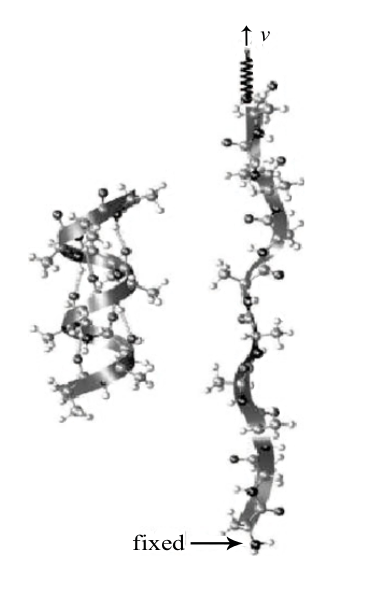
\includegraphics[scale=0.5]{pulling}
		\caption{Pulling experiment on a small peptide (Tuckerman, pg 328)}
		\label{fig:pulling}
	\end{figure}

The idea is to fix an end of the peptide and pull the other end, for example with optical tweezers in an experimental setting (shown in picture \ref{fig:pulling}.
Computationally, a time-dependent potential drives the end-to-end distance $|\vec{r}_1-\vec{r}_N|$ of a peptide away form its equilibrium value in the folded state:

$$U(\vec{r}_1, \dots, \vec{r}_N, t) = U_o(\vec{r}_1, \dots, \vec{r}_N) + \frac{1}{2}k\bigl(|\vec{r}_1-\vec{r}_N|-r_{eq}-vt\bigr)^2$$

We have a potential to describe the system and a harmonic term.
The pulling is performed at speed $v$.

Ensemble of initial conditions with different pulling rates.

$$\langle e^{-\beta\mathcal{W}_{AB}}\rangle_A = e^{-\beta\Delta A_{AB}}$$

The estimate gets better with the number of simulations performed. 

There are several problems, for example work values have a distribution $P(\mathcal{W}_\tau)$, as shown in figure \ref{fig:dist}.

\begin{figure}[H]
		\centering
		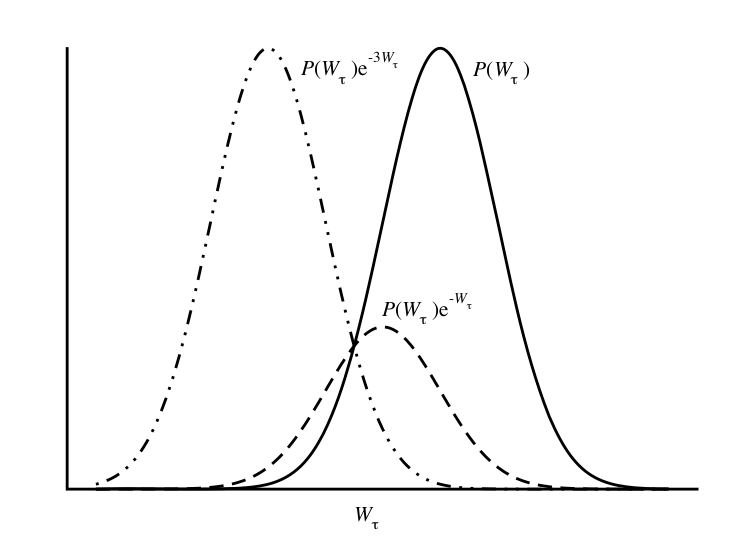
\includegraphics[scale=0.5]{dist}
		\caption{Shift in a Gaussian work distribution as a result of the multiplication by $exp(- \beta W_{\tau})$ for various values of $\tau$.}
		\label{fig:dist}
	\end{figure}	


We need to be very careful with defining the quantity 

$$\langle e^{-\beta\mathcal{W}_\tau}\rangle= \int\mathcal{W}_\tau P(\mathcal{W}_\tau)e^{-\beta\mathcal{W}_\tau}$$

There are however some tricks we can perform. For example if, and only if, we know $P(\mathcal{W}_\tau)$ is Gaussian:

$$\ln\langle e^{-\beta\mathcal{W}_\tau}\rangle\simeq-\beta\langle\mathcal{W}_\tau\rangle + \frac{\beta^2}{2}(\langle\mathcal{W}_\tau^2\rangle-\langle\mathcal{W}_\tau\rangle^2)$$

Also, we are not sure that at the end the system reaches equilibrium. 
If the force is too strong we are forcing the system out of equilibrium and we'll not reach convergence.

\section{Replica exchange Monte Carlo}
Replica ex change Monte Carlo is not a free energy calculation method.
However, in the case of proteins, the free energy profile is complicated, with a lot of free energy minima and maxima (\textbf{rough free energy profile}), like the one in figure \ref{fig:rough}.

\begin{figure}[H]
		\centering
		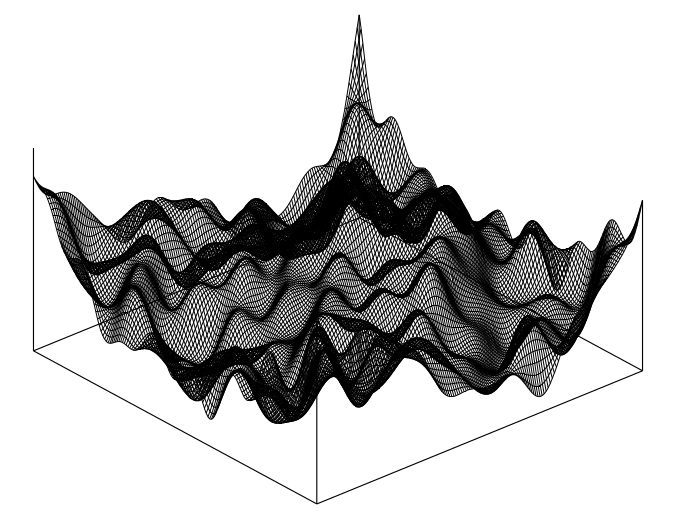
\includegraphics[scale=0.5]{rough}
		\caption{A two-dimensional rough potential energy surface.}
		\label{fig:rough}
	\end{figure}

The problem with exploring such complicated potentials is the high probability of gettin stuck in a minimum.
The way out of this is to build $M$ independent copies of a system: each replica is assigned a different value of some physical control variable or parameter.
The simulations are performed independently from each other, but at a certain time we try to go from one replica to another.
There are several methods to perform these "jumps".

	\subsection{Parallel tempering}
	$M$ independent copies of a system: $T_M>T_{M-1}>T_{M-2}>\cdots>T_1$, where $T_1$ is the temperature of the canonical distribution to be sampled.
	
	\begin{figure}[H]
		\centering
		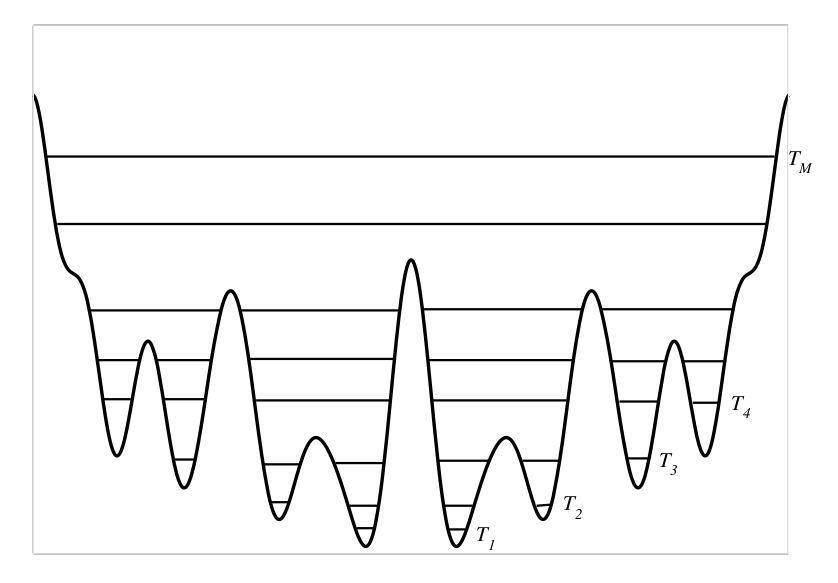
\includegraphics[scale=0.5]{RE}
		\caption{Schematic of the parallel-tempering replica exchange Monte Carlo.}
		\label{fig:RE}
	\end{figure}
	
	At temperature $T_M$ we can sample everywhere, but every now and then we want to try to switch coordinates.
	
	Configuration of replicas $\vec{r}^{(1)}, \dots, \vec{r}^{(M)}$.
	Independent replicas: total probability distribution:

	$$F(\vec{r}^{(1)}, \dots, \vec{r}^{(M)}) = \prod\limits_{K=1}^Mf_K(\vec{r}^{(K)})\qquad f_K(\vec{r}^{(K)}) = \frac{e^{-\beta_K U(\vec{r}^{(K)})}}{Q(N ,V, T_K)}$$

	Select randomly two neighboring replicas and attempt replica exchange:

	$$(\vec{r}^{(K)}, \vec{r}^{(K+1)})\rightarrow (\tilde{\vec{r}}^{(K)}, \tilde{\vec{r}}^{(K+1)})\qquad\text{ with }\qquad \tilde{\vec{k}}^{(K+1)} = \vec{r}^{(K)}\land \tilde{\vec{r}}^{(K+1)}=\vec{r}^{(K)}$$

	Coordinates are merely exchanged:

	$$T(\tilde{\vec{r}}^{(K)}, \tilde{\vec{r}}^{(K+1)}|\vec{r}^{(K)}, \vec{r}^{(K+1)}) = T(\vec{r}^{(K)}, \vec{r}^{(K+1)}|\tilde{\vec{r}}^{(K)}, \tilde{\vec{r}}^{(K+1)})$$
	
	The $T$ is the trial probability for a move that takes the system from coordinates $vec{r}^{(K)}, \vec{r}^{(K+1)}$ to the coordinates $\vec{r}^{(K)}, \vec{r}^{(K+1)}$. 

	The acceptance probability is given by the metropolis rule:

	$$A(\tilde{\vec{r}}^{(K)}, \tilde{\vec{r}}^{(K+1)}|\vec{r}^{(K)}, \vec{r}^{(K+1)}) = A(\vec{r}^{(K+1)}, \vec{r}^{(K)} | \vec{r}^{(K)}, \vec{r}^{(K+1)})$$
	
	The probability for a new state is given by  $f_K(\vec{r}^{(K+1)})f_{K+1}*\vec{r}^{(K)}$. 
	
	$$A(\vec{r}^{(K+1)}, \vec{r}^{(K)} | \vec{r}^{(K)}, \vec{r}^{(K+1)}) = \min\biggl[1, \frac{f_K(\vec{r}^{(K+1)})f_{K+1}*\vec{r}^{(K)}}{f_K(\vec{r}^{(K)})f_{K+1}(\vec{r}^{(K+1)})}\biggr] = \min[1, e^{-\Delta_{K, K+1}}]$$

	$$\Delta_{K, K+1} = (\beta_k-\beta_{K+1})[U(\vec{r}^{(K+1)}) - U(\vec{r}^{(K)})]$$\footnote{In the Tuckerman these two terms have opposite sign.}
	
	Some switches of replicas can be done up high, meaning the system will \textit{percolate}, that will therefore go through barriers in this way.
	
	\subsection{Wang-Landau sampling}
	The Wang-Landau sampling is a clever way to build the partition function at any possible temperature by simply running a simulation: \textbf{iterative method}.

	The partition function can be derived by using Boltzmann weights and the densities of states (how many states are there at energy $E$): 
	$$Q(N, V, T) = \frac{1}{E_0}\int_0^{\infty}dEe^{-\beta E}\Omega(N, V, E)\Rightarrow Q(\beta) = \int_0^{\infty}dEe^{-\beta E}\Omega(E)$$
	
	The partition function becomes an integral over all values of energy of the function given by the Boltzmann factor and the density.
	
	The idea is to obtain directly $\Omega(E)$, the inverse of the probability of state $E$.
	Assign $\Omega(E)=1\forall E$ (discredited), meaning all energy values are equally probable (which is not really the case).
	Then a trial move is performed: $E_1\rightarrow E_2$ and it is accepted by the metropolis rule:

	$$A(E_2|E_1) = \min\biggl[1, \frac{\Omega(E_1)}{\Omega(E_2)}\biggr]$$

	After each move: $\Omega(E)\rightarrow \Omega(E)f\quad f>1$.
	If we visit one particular value of the energy, then the density of states for that value will increase.
	Thus meaning that the probability of visiting again that state will decrease.
	
	We can build the histogram $h(E)$ of visited states, that will become always more flat with time.
	Once $h(E)$ is flat enough a new value $f_{new} = \sqrt{f_{old}}$ is switched and the algorithms continue until convergence.
	There is no detailed balance due to $f$.
	
	
	
	
	
	
	
	
	
	
	
	
	
	
	
